\documentclass{article}
\usepackage[utf8]{inputenc}

\title{Neural Machine Translation by Jointly Learning to Align and Translate}
\author{}
\date{}

\usepackage{natbib}
\usepackage{graphicx}
\usepackage{amsmath}
\usepackage[left=2.5cm,right=2.5cm,top=1cm,bottom=1.25cm]{geometry}
\usepackage{hyperref}
\usepackage{float}
\usepackage[export]{adjustbox}



\hypersetup{colorlinks=true,urlcolor=blue}
\pagenumbering{gobble}

\begin{document}

\maketitle

\section*{Link}
\href{https://arxiv.org/abs/1409.0473}{arXiv} 

\section*{Summary}
\begin{itemize}
    \item One limitation of encoder-decoder architecture in machine translation is that encoder neural network needs to be able to compress all the necessary information of a source sentence into a fixed length vector. This causes the performance of such model to degrade rapidly when the length of the input sentence increases. To overcome it, this paper proposes a model which learns to align and translate jointly. It encodes the input sentence into a sequence of vectors and chooses a subset of these vectors adaptively while decoding the translation. 
    \item When generating a target word, the context vector is computed as a weighted sum of encoder hidden states. The weights for the alignment model is learned jointly with the translation model.
    \begin{figure}[H]
        \centering
        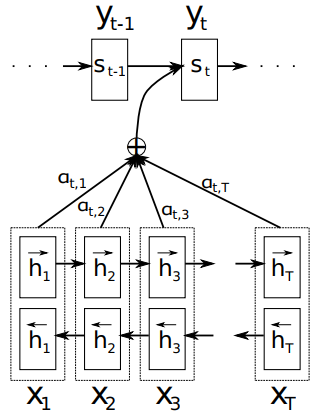
\includegraphics[scale=0.45]{attention.png}
        \caption{Attention model}
        \label{fig:Figure 1}
    \end{figure}
    \item The proposed attention based model which uses bidirectional RNN outperforms the conventional encoder-decoder based model. The performance of this model is not affected by longer source sentence unlike previous models.
     \begin{figure}[H]
        \centering
        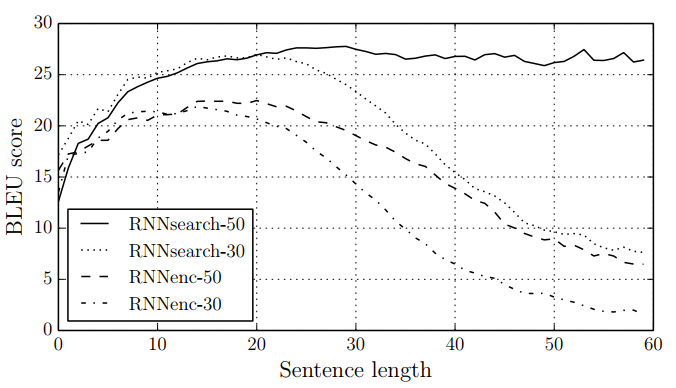
\includegraphics[scale=0.45]{performance.png}
        \caption{Performance of attention model(RNNsearch-50 is much better than the model without attention (RNNenc-50) and stable for long sentences}
        \label{fig:Figure 1}
    \end{figure}   
    \item The alignments learn by the model shows that it can learn non-trivial and non-monotonic alignment between source and target sentence.
    \item For each iteration the time required is proportional to the length of the longest sentence in the minibatch. To minimize waste of computation, before every 20-th update, they retrieved 1600 training pairs, sorted them according to the lengths and split them into 20 minibatches.  

    
\end{itemize}

\end{document}
